\chapter{Sleep Apnea}

Sleep apnea is a disorder where breathing stops and starts repeatedly during sleep. Stop breathing happens when either the airway collapses or the brain can not successfully send the signal to the breathing muscles. The first case is called Obstructive Sleep Apnea (OSA), and the second case is called Central Sleep Apnea (CSA). In both cases no air come in or out of the lung. It often lasts from a few seconds to minutes, and can happen about 30 times or more per hour\cite{NHLBI}. Sleep apnea is difficult to diagnose, because it happens when the patient sleeps. Moreover, sleep apnea can not be detected by normal tests such as blood test. It can be noticed by a family member when the patient intensively snores. However, CSA does not often come with snoring, therefore there it is difficult to detect sleep apnea in general. Sleep apnea can lead to many serious diseases if it is untreated, such as high blood pressure, heart attack, stroke, heart failure, etc. Getting not enough sleep can cause serious accidents if truck or taxi drivers have this disease. Section 2.1 presents a taxonomy of sleep apnea. Section 2.2 describes the physiological signals that can be used to diagnose sleep apnea.

\section{Taxonomy of sleep apnea}
Sleep apnea is more dangerous than people have thought, because it can lead to many other well-known diseases. According to The Akershus Sleep Apnea Project, there are 25\% middle-aged Norwegians at high-risk of having OSA\cite{Akershus}. That means sleep apnea is very common and it has to be studied seriously. In fact, there are dozen of research papers about it. When searching with "sleep apnea" on Google Scholar, it returns about about 18900 related articles. Sleep apnea is divided into three types:

\begin{itemize}
  \item OSA occurs when the soft tissue falls to the back of the throat which causes the breathing to be obstructed during sleep.
  \item CSA occurs when the brain fail to sends the signals to the breathing muscles and therefore it fails to control the breathing cycle.
  \item Mixed sleep apnea (MSA) is a combination of both OSA and CSA.
\end{itemize}

\subsection{Central sleep apnea}
    \textit{``Central sleep apnea syndrome is characterized by a cessation or decrease of ventilatory effort during sleep and is usually associated with oxygen desaturation."}\cite{Westchester}
    
    CSA happens when the brain can not send the appropriate signals to muscles which control breathing. CSA is not as common as obstructive sleep apnea. CSA is sometime a consequence of other diseases like heart failure, stroke, or sleep at high altitude.\\\\
    \textbf{Symptoms:} Common symptoms of CSA are awakening suddenly with breathlessnesses, insomnia, headache in the morning, difficulties to focus on work, hypersomnia, or snoring. The bed-partner can notice that the patient may stop breathing a number of times during sleep, about 30 times or more per hour, and the patient may snore. However, snoring is not common in CSA, and snoring does not always mean that a patient has sleep apnea.\\\\
    \textbf{Causes:} There are many causes that make the brain fail to connect with the breathing muscles. One of them is Cheney-Stokes, which is often associated with congestive heart failure or stroke, and is characterized by rhythmic cycles gradually increased and then decreased breathing which results in a temporary pause in breathing. 
    Other reasons which cause central sleep apnea are certain medical conditions. For example, if a patient has problem in cerebrovascular or has brain tumors can cause that signals to the breathing system get lost. Certain drugs such as opium, morphine or codeine can lead to irregular breathing like increase, decrease or stop breathing. Sometime sleep at high altitude can cause central sleep apnea, but it is not a big problem, because the problem will disappear when moving to a lower altitude.\\\\
    \textbf{Complications:} Not getting enough sleep can cause cardiovascular diseases. When the oxygen level in the blood is low, the heart will work hard to deliver blood to the tissues. If this lasts for a long time it may cause heart failure. Likewise, when the heart works hard, the pressure on the vascular increases which can cause hypertension. Hypertension is one of the most dangerous diseases and can lead to stroke or even dead. Waking up many times at night will make us tired and difficult to restore normal sleep. People who do not get enough sleep often have severe daytime sleepiness, fatigue and irritability. They can not focus on work and sometime fall asleep, not only at work but also when they drive a car.\\\\
    \textbf{Diagnostic methods:} Usually a doctor may perform an evaluation based on those symptoms which are mentioned above, or a patient must be sent to a treatment center for sleep disorders. At the treatment center, the patient can be analyzed by overnight monitoring breathing and other body functions during sleep. In polysomnography testing, the patient is connected to monitoring devices such as heart, lung, brain activity, breathing patterns, arm and leg movement, blood oxygen during levels sleep. Moreover, a review by a cardiologist or a doctor who specializes in the nervous system may also necessary to find the causes of central sleep apnea.\\\\
    \textbf{Treatments:} The first step of treatment is to try to cure the other diseases which cause the central sleep apnea. For example, a good treatment of a heart failure may eliminate central sleep apnea. The other way to treat this disease is to use drugs. There are some drugs which have been used to stimulate breathing for those who have central sleep apnea. For example, acetazolamide can be used to prevent central sleep apnea at high altitude. However, other drugs can cause apnea, for example opioid. The dose of opioid drugs need to be reduced if it causes central sleep apnea. However, drugs are not the major solution to treat central sleep apnea. \\There are four physical treatment methods which are often used in treating central sleep apnea. The first one is continuous positive airway pressure (CPAP), which uses mild air pressure to keep the airway open. This treatment is mainly used for obstructive sleep apnea where the patient wears a mask on the nose during sleep, but it is also used for central sleep apnea. Another useful method is bilevel positive airway pressure (BPAP) which supplies stable and continuous pressure in the upper airways while breathing in and out. BPAP provides high pressure when inhaling and low pressure when exhaling. The purpose of this treatment is to boost the weak breathing pattern of central sleep apnea into normal. Some BPAP devices can detect if there is no air-follow in a few seconds it will automatically active the breathing system. There is a better solution than CPAP and BPAP, that is called adaptive servo ventilation (ASV). ASV is designed to treat central sleep apnea and complex sleep apnea by monitoring normal breathing pattern and storing it in a database system as a training set. When the patient falls asleep, ASV monitors the breathing process and compares it with the training set. If there is apnea, ASV will use pressure to regulate the breathing pattern and prevent pause in breathing. The last method is using supplemental oxygen, but there are many arguments against this method. The main argument is that the oxygen level may normalize, but the carbon dioxide can not release. As a result, a signal will be sent to brain which causes awakenings and the sleep will be fragmented. 
\subsection{Obstructive sleep apnea}
    \textit{``Obstructive sleep apnea syndrome is characterized by repetitive episodes of upper airway obstruction that occur during sleep, usually associated with a reduction in blood oxygen saturation."}\cite{Westchester}
    
    Several types of sleep apnea exist, but the most serious and common type is obstructive sleep apnea. It occurs when the throat muscles relax and blocks the airway during sleep. The most noticeable signal of obstructive sleep apnea is snoring, although not everyone who snores has obstructive sleep apnea. It usually affects old people, but anyone can have this illness. Obstructive sleep apnea is particularly common for those who are overweight. We discuss more in detail about its symptoms, causes, complications, diagnostic methods, and treatments below.\\
    \textbf{Symptoms:} As mentioned above, the most common signs is loud snoring and sometimes pausing in snoring. When there is a pausing in snoring, choking and gasping may follow it. Apnea occurs when the throat muscles relax and block the airway, therefore when we sleep on our back the snoring will be loudest. When we turn on our side, the snoring sound will decrease or even stop. That explains why we do not snore every night. It is difficult for us to recognize that we are snoring. However, a family member can easily notice the problem. Another sign is that we have excessive sleepiness during the day, can fall asleep while working, watching television or even driving. When we do not have normal breathing at night, our brain does not have enough oxygen to work. It causes not only morning headaches, but also memory problems. The other good sign to detect obstructive sleep apnea is waking up with dry mouth or sore throat.\\
    \textbf{Causes:}
    The airway composes of mouth, nose, throat, and windpipe. It always opens under sleep when we do not have sleep apnea. 

    \begin{figure}[h]
        \centering
        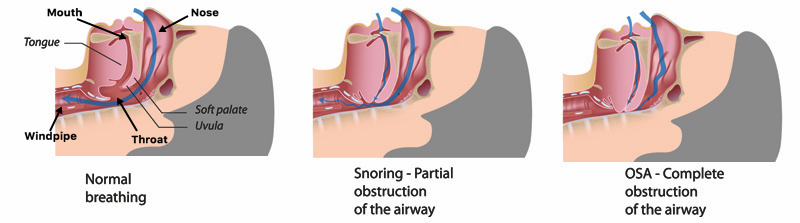
\includegraphics[width=1.0\textwidth]{Figures/ObstructionVentilationApnea.png}
        \caption{Obstructive Sleep apnea \cite{HudsonOSA}}
        \label{fig:Figures/ObstructionVentilationApnea}
    \end{figure}
    However, the airway becomes narrow when the soft palate and uvula relax. As a result, it is difficult to breath, and the patient might snore. This is called partial obstruction of the airway. When the muscles in the back of the throat relax too much, they will block the airway, as a result normal breathing is impossible. This situation is called complete obstruction of the airway, or obstructive sleep apnea. Blocked in breathing may cause a lower oxygen level in blood. Hence, the brain sends a signal to wake up the patient that the airway can be reopened. This process usually happens in a very short time and it is often not noticed because shortness of breath may be fixed with one or two deep breaths.\\ 
    Major causes of obstructive sleep apnea are old age, brain injury, decreased muscle tone, increased soft tissue around the airway, obese, or structural features that give rise to a narrowed airway\cite{OSAWiki}. Everyone can have obstructive sleep apnea, but certain factors imply a higher risk. The most significant factor is excess weight. Over a half of the people with OSA are overweight, because the fat of the upper respiratory can block breathing. The size of the neck may indicate whether someone at risk of OSA or not, because a thick neck can narrow the airway. Other risk factors are alcohol and smoking. Mihaela Trenchea et.al have researched on this topic and showed that smokers who smoke more than one pack  of cigarettes a day are at higher risk of severe obstructive sleep apnea than those who do not smoke\cite{ChestWorldCongress}. Other minor but not least causes are sex, age, genetic, or race. Overall, men are twice likely to develop OSA than women, and older have this illness more often than younger.\\
    \textbf{Complications:} Obstructive sleep apnea is a serious health problem which leads to several complications like:\\
    \textit{Cardiovascular diseases.} As mentioned in central sleep apnea complications, when the tissues do not get enough oxygen, the heart will beat fast and hard. As a result, the pressure on the heart and vascular will increase. About half of people with sleep apnea have high blood pressure, which increases the risk of heart failure and stroke. The more serious obstructive sleep apnea, the higher the risk of high blood pressure. With an underlying heart disease, a repeated low blood oxygen level can lead to sudden death from a cardiac event. Moreover, people with obstructive sleep apnea are often capable of developing abnormal heart rhythms like atrial fibrillation. \\\\
    \textit{Medications and surgery.} In general anesthesia, the doctor will use some medications like narcotic analgesics which can relax the patient's upper airway. When patient lies on his back, it will cause severe problems. Therefore it is important that patients with obstructive sleep apnea or related symptoms must inform the physician.\\\\
    \textit{Tired and sleepiness at daytime.} Similar to central sleep apnea, daytime drowsiness, fatigue and irritability are results from repeatedly awaking at night. Moreover, people with obstructive sleep apnea have often difficulties to focus on work or driving. Hence, it is not only dangerous for the patient, but also dangerous for people who are around him.\\\\
    \textit{Partner's insomnia.} Snoring may be a huge problem for those who have to listen to it. Sleeping with a snoring bed partner sometime is a nightmare, because the people who do not snore can be woken up by the snoring sound. As a result, the partner may get some health problem related to insomnia. In some cases, the partner may leave sharing room to find a quiet place to sleep, or even it is a cause for divorce.\\\\
    
    \textbf{Diagnostic methods:}
    The evaluation may usually be performed by observing signs and symptoms. Then some tests need to be done, such as measuring the neck or checking the blood pressure. The medical doctor may examine the back of the throat, mouth and nose to find out if there are any abnormalities. Further evaluation requires to stay overnight at a sleep center. At that place, breath and other body functions are monitored while the patient is sleeping.\\\\
    \textit{Sleep tests.} 
    A patient may be asked to stay at a clinic for monitoring the heart, lung, brain activity, body movements, breathing patterns, and blood oxygen levels during sleep by using professional devices. Based on the information from those sensors, the physician can diagnose obstructive sleep apnea and its level of severeness. Sometimes a patient has other diseases which also have the same symptoms as obstructive sleep apnea. For example, narcolepsy also causes excessive daytime sleepiness, but does not have the same treatment.\\\\
    \textit{Measuring oxygen.} 
    The patient does not need to come to a sleep center. Instead, a small sensor which can measure the oxygen level in blood can be used. The patient can stay at home and wear this sensor on his finger to carry out the measurement. It is very simple, consistent and painless. While the patient sleeps, the sensor collects the information about oxygen level, and may store it on a computer or smart phone. Then the data will be sent to the physician. Based on the pattern of oxygen level in blood, the physician can determine if the patient has obstructive sleep apnea, or the patient may be recommended a sleep test at a sleep center.\\\\
    \textit{Otolaryngology tests.}
    This is often performed when a patient snores too loud. As mentioned earlier, when someone snores, it does not mean that he has obstructive sleep apnea. However, over a half people who snore have this illness. Hence, examinations on the nose, mouth, throat, palate, and neck need to be carried out.\\\\ 
    \textit{Cardiopulmonary tests.} 
    These tests usually relate to the measurements of the air flow, the breath samples and the heart rate samples. By observing the heart rate and respiration from the abdomen and chest, the physician can determine whether the patient has obstructive sleep apnea or not. 

    \textbf{Treatments:} We can apply three types of treatments which are lifestyle changes, therapies, and surgery or other procedures \cite{MAYOCLINIC}.\\
    \textit{Lifestyle changes.}
    This is the first  treatment to try when OSA is diagnosed. Half of people who have obstructive problem are obesity, hence trying to loose weight is the first thing to do for the overweighted patients. Beside weight-loss, avoiding alcohol is helpful, since alcohol can also cause this illness. Therefore, one should not drink too much alcohol, especially several hours before bed \cite{MAYOCLINIC}. Obstructive problem is happened when the airway at the throat collapses. Therefore, it is better to lie on the side instead of lying on the back.\\\\
    \textit{Therapies.} The methods applied for central sleep apnea are also applied for OSA, normally are CPAP, BPAP and ASV.\\\\
    \textit{Surgery.}
    The goal of surgery is to remove the excess tissue from the throat which can collapse and block the airway. There are several surgical options: surgical opening in the neck, surgical removal of tissue, jaw surgery, upper airway stimulation, and implants \cite{MAYOCLINIC}.
\subsection{Mixed sleep apnea}
    Mixed sleep apnea is also known as complex sleep apnea. It is a merger of central sleep apnea and obstructive sleep apnea. It is identified by researchers at Mayo Clinic \cite{ScienceDaily}. Mixed sleep apnea is caused when the respiratory control is interfered. Namely, the brain sends a signal to control the breathing system, but the responses of the breathing are not as the brain desired. When using CPAP, it can cause chaos on the ventilator control. As a result, obstructive sleep apnea can be cured, but the central sleep apnea can occur because the signals which are sent to the breathing system do not work. New CPAP devices can supply additional carbon dioxide to stabilize the breathing pattern to avoid mixed sleep apnea \cite{Hindawi}.
\section{Observable characteristics of obstructive sleep apnea}

    By examining the sensors' abilities of observing the signals which can be used to observe obstructive sleep apnea, we suggest to divide those signals into two categories. The first group comprises signals that can be simply measured by sensors which are integrated in smart wearable devices. The other group includes complex signals which can only be obtained by professional devices and can be transfered to user devices. Simple signals are the heartbeat, the change the volume of the chest and abdomen, and snoring. The complex signals include EEG, EMG, EOG, ECG, oxygen saturation in the blood, breathing, and blood pressure. Some non-professional devices can also obtain these signals. However, the results from them are not good enough to use for medical diagnosis. For instance, the BITalino can observe almost all of the complex signals, but it is not a medical device as disclaimer on the BITalino website.

    \begin{figure}[h]
        \centering
        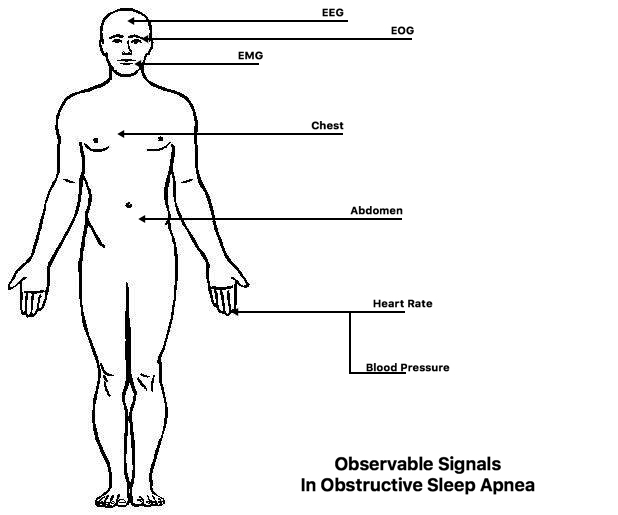
\includegraphics[width=1.0\textwidth]{Figures/humanbody.jpg}
        \caption{Observable Signals \cite{Advan}}
        \label{fig:Figures/humanbody}
    \end{figure}

    
    \textbf{Heartbeat. } The normal heart rate of a person varies from 60 to 100 beats per minute \cite{HEARTORG_HR} depending on how often that person trained. Hence, each person has a stable heart rate in this range. However, sleep apnea causes the heart rate to increase and to break the ordinary pattern. Heart rate is usually easily measured by using a smart watch or smart ring, or even a tattoo circuit. These devices can collect data and may send it to a smart phone to analyze it.

    \textbf{Snore. } Snoring can be measured by the microphone of a smart phone. The received signal is compared with available data samples. The result of the comparison can be used to determine whether the snoring is related to OSA or not. Snoring is often stopped after a period of time when people awake and start snoring again.

    \textbf{Measure the volume of air to breathe.} When observing the movement of the chest with a camera phone, Reyes gave Bersain\cite{BersainReyes} can calculate the average respiratory rate and tide volume.

    In addition to the signals which can be measured by integrated sensors on the smart devices, we can keep track of OSA by using non-integrated sensors to measure signals such as electroencephalogram (EEG), electromyography (EMG), electrooculography (EOG), electrocardiography (ECG), oxygen saturation in the blood, nasal airflow, and blood pressure.\\

    \textbf{EEG. } Wafaa S. Almuhammadi et.al\cite{IEEEOSAEEG} have done research on using EEG to classify OSA. They used EEG signals from Physionet as input for mining methods to detect if OSA exists or not. However, using only EEG for detecting OSA is not a good idea, because there are many health problems that have similar symptomatology to OSA, and one of them is epileptic \cite{NCBIEGEPILEPSY}. EEG can be recorded by placing the electrodes along the scalp, which is uncomfortable compared to wearing smart devices. However, EEG is very useful in combination with the others observable signals. In other words, EEG is considered an important signal for detecting OSA.\\\\
    \textbf{EMG. }People with OSA usually have longer time for the tongue to be recovered from relaxed. By examining the genioglossus muscle activity useful data for OSA diagnosis can be collected. Marc B Blumen et.al \cite{SDEMG} have found that those with OSA have tongue recovery time much longer than normal people after a constant submaximal effort, and they also have a smaller decrease in genioglossus muscle median frequency during effort. For OSA, we focus only on the signals from the tongue and genioglossus muscle because it causes the airway to be blocked. Other EMG signals are not considered, because they are not relevant.\\\\
    \textbf{EOG. }To measure eyes movements during sleep electrooculography is used. Electrooculography has two electrodes. The front of the eyes, also known as the cornea, is electrically positive while the back, also known as the retina, is electrically negative. Therefore, it is possible to measure the variation in voltage to determine the movements of the eyes. Rapid eye movement (REM) is a factor in the occurrence of disordered breathing events\cite{JSREM}. \\\\
    \textbf{ECG. } ECG presents the electrical activity of the heart, and it is one of the most efficient signal to detect OSA. By placing the electrodes on the skin, the tiny electrical changes on skin during each heartbeat can be detected. Laiali Almazaydeh et.al \cite{RESEARCHGATE} have done research on detecting OSA by using ECG signal features. They observe the wave forms from ECG, then identify an R peak. Once R peak is identified, they calculate RR intervals. After extracted, RR intervals are submitted to SVM in order to do classification.\\\\
    \textbf{Oxygen saturation. } Oxygen saturation can be measured by using pulse oximetry. Pulse oximetry is a noninvasive and inexpensive procedure which is used to measure the level of oxygen in blood. It is very simple to make measurements, a clip-like sensor can be placed on the earlobe, nose or fingers\cite{WIKIHOW}. The level of oxygen in the blood is usually above 95\%.\\\\
    \textbf{Nasal airflow. } Airflow sensors can measure the air pressure in nose when inhaling and exhaling. The sensor can be easily placed, but it is uncomfortable to wear it during sleep. A lot of studies have reported that it is not a good signal for detecting OSA, but it is still used\cite{HINDIWAAIRFLOW}. Therefore, we consider nasal airflow as one of signals to detect OSA.\\\\
    \textbf{Blood pressure. } Blood pressure can be measured by a simple, noninvasive sensor. This sensor can easily clip on the finger. According to American Heart Association\cite{HEARTORG}, the normal blood pressure with systolic is less than 120 mm Hg, and with diastolic is less than 80 mm Hg. Getting higher number than these numbers when sleeping is considered having OSA. As explained in OSA causes, the pressure is high when the breathing pauses.\\


